% ----------------------------------------------------------------------
%                   LATEX TEMPLATE FOR PhD THESIS
% ----------------------------------------------------------------------

% based on Harish Bhanderi's PhD/MPhil template, then Uni Cambridge
% http://www-h.eng.cam.ac.uk/help/tpl/textprocessing/ThesisStyle/
% corrected and extended in 2007 by Jakob Suckale, then MPI-CBG PhD programme
% and made available through OpenWetWare.org - the free biology wiki
% and finally modified in 2015-2017 by Holger Nahrstaedt
% https://github.com/holgern/TUB_PhDThesisTemplate

%: Style file for Latex
% Most style definitions are in the external file PhDthesisTUB.
% In this template package, it can be found in ./Classes/

\documentclass[twoside,11pt,online,a4paper,pdfa1,custommargin,numbered,customfont]{PhDthesisTUB}
 

% *********************** Choosing pdfx standard ******************************
% `pdfa1'
% `pdfa2'
% `pdfx3'
% *********************** Change Thesis-Language to German ******************************
% default is english
% `german' : language is set to german
%
% % *********************** Choosing oneside / twoside ******************************
% `oneside' : layout is optimized for one-side print
% `twoside' : layout is optimized for two-side print
% *********************** Choosing print / online ******************************
% `print' : pdf-file is optimized for print
% `online' : pdf-file is optimized for online submission. The links are colorfull.
% *********************** Choosing biblatex or bibtex ******************
% `biblatex' : biblatex is used. Biblatex is automatically set when using xetex
%
% *********************** Choosing bibliographystyle ******************
% `numbered' : (default option) e.g. [1], [2]
% `authoryear' :  e.g. Name (2008)
% `custombib' : Use your own style, which is defined in preamble.tex
% *********************** Choosing the Fonts size ******************
% `9pt'
% `10pt'
% `11pt'
% `12pt'
% *********************** Choosing the paper size ******************
% `letterpaper'
% `a4paper'
% `a5paper'
% *********************** Choosing the Fonts in Class Options when using pdflatex ******************
% 
%  On Windows, the packge cm-super has to be installed!
%
% `' :  computer modern
% `fontA' :  newtxmath
% `fontB' :  cmbright
% `fontC' :  libertine,newtxmath
% `fontD' :  concmath
% `fontE' :  iwona
% `fontF' :  kurier	
% `fontG' :  anttor
% `fontH' :  kmath,kerkis
% `fontI' :   mathdesign (Utopia)
% `fontJ' :  fouriernc
% `fontK' :  pxfonts
% `fontL' :  mathpazo
% `fontM' :  mathpple
% `fontN' :  txfonts
% `fontO' :  mathtime (Belleek)
% `fontP' :  mathptmx	times	
% `fontQ' :  mbtimes	omega
% `fontR' :  arev
% `fontS' :  mathdesign (Charter)	
% `fontT' :  comicsans
% `fontU' :  mathdesign (Garamond)
% `fontV' :  fourier	utopia
% `fontW' :  ccfonts,eulervm
%
% `customfont': Use `customfont' option in the document class and load the
% package in the preamble.tex
%
% default or leave empty: `Latin Modern' font will be loaded.
%
% *********************** Choosing the Fonts in Class Options when using xelatex/lualatex ***********
%
% `' :  computer modern
% `fontA' :  XITS - XITS Math
% `fontB': Cambria - Cambria Math
% 'fontC': Libertinus - Libertinus Math
% 'fontD': TeX Gyre Pagella - Asana Math
% 'fontE': TeX Gyre Pagella - TeX Gyre Pagella Math
% 'fontF': TeX Gyre Schola - TeX Gyre Schola Math
% 'fontG': TeX Gyre Termes - TeX Gyre Termes Math
% 'fontH': TeX Gyre Bonum - TeX Gyre Bonum Math
% 'fontI': DejaVu Sans - TeX Gyre DejaVu Math
%
% `customfont': Use `customfont' option in the document class and load the
% package in the preamble.tex
%
% default or leave empty: `Latin Modern' font will be loaded.
%
% ************************* Custom Page Margins ********************************
%
% `custommargin`: Use `custommargin' in options to activate custom page margins,
% which can be defined in the preamble.tex. Custom margin will override
% print/online margin setup.
%
% ************************* other options ********************************
% `abstract`: Only the title-page and the abstracts are generated
%

\usepackage{todonotes}
\usepackage{acronym}
%%% Needed packages for commands

\usepackage{xcolor}
%\usepackage{amsthm}
\usepackage{mathtools}
%%% Mathematics

%% Miscellaneous

\newcommand{\uptoconst}{\mathrel{\overset{\makebox[0pt]{\mbox{\normalfont\small\sffamily c}}}{=}}}
\newcommand{\half}{\frac{1}{2}}
\def\*#1{\mathbf{#1}}

%% Analasis

\newcommand{\real}{\mathbb{R}}
\newcommand{\grad}{\nabla}

%% Linear Algebra

\newcommand{\logdet}[1]{\log\left|#1\right|}
\newcommand{\trace}{\text{tr}}
\newcommand{\diag}{\mathrm{diag}}
\newcommand{\dt}[1]{\frac{d#1}{dt}}
\newcommand{\deriv}[2]{\frac{d#1}{d#2}}

%% Matrices

\newcommand{\Knm}{K_{nm}}
\newcommand{\invKmm}{K_{mm}^{-1}}
\newcommand{\Ktilde}{\widetilde{K}}
\newcommand{\invKtilde}{\widetilde{K}^{-1}}

%% Probabilities

\newcommand{\PG}{\text{PG}} % Polya-Gamma
\newcommand{\Po}{\text{Po}} % Poisson
\newcommand{\No}{\mathcal{N}} % Normal
\newcommand{\GP}{\mathrm{GP}} % GaussianProcess
\newcommand{\Ga}{\mathrm{Ga}} % Gamma
\newcommand{\NB}{\mathrm{NB}} % Negative Binomial
\newcommand{\KL}[2]{\mathrm{KL}\left(#1\vert\vert #2\right)} % KL Divergence
\newcommand{\IG}{\mathrm{IG}} % Inverse Gamma
\newcommand{\Be}{\mathrm{Bernoulli}} % Bernoulli
\newcommand{\GIG}{\mathrm{GIG}} % Generalized Inverse Gaussian
\newcommand{\EE}{\mathbb{E}}
\newcommand{\dd}{\mathrm{d}}
\newcommand{\RR}{\mathbb{R}}
\newcommand{\ELBO}{\mathcal{L}}
\newcommand{\VFE}{\mathcal{F}}

%% Symbols

\newcommand{\bX}{\boldsymbol{X}}
\newcommand{\bO}{\boldsymbol{O}}
\newcommand{\bZ}{\boldsymbol{Z}}
\newcommand{\bD}{\boldsymbol{D}}
\newcommand{\bx}{\boldsymbol{x}}
\newcommand{\boldf}{\boldsymbol{f}}
\newcommand{\boldg}{\boldsymbol{g}}
\newcommand{\boldy}{\boldsymbol{y}}
\newcommand{\boldz}{\boldsymbol{z}}
\newcommand{\by}{\boldsymbol{y}}
\newcommand{\bn}{\boldsymbol{n}}
\newcommand{\bu}{\boldsymbol{u}}
\newcommand{\boldu}{\boldsymbol{u}}
\newcommand{\boldm}{\boldsymbol{m}}
\newcommand{\boldn}{\boldsymbol{n}}
\newcommand{\bgamma}{\boldsymbol{\gamma}}
\newcommand{\bomega}{\boldsymbol{\omega}}
\newcommand{\bOmega}{\boldsymbol{\Omega}}
\newcommand{\blambda}{\boldsymbol{\lambda}}
\newcommand{\bSigma}{\boldsymbol{\Sigma}}
\newcommand{\bdelta}{\boldsymbol{\delta}}
\newcommand{\btheta}{\boldsymbol{\theta}}
\newcommand{\bbeta}{\boldsymbol{\beta}}
\newcommand{\balpha}{\boldsymbol{\alpha}}
\newcommand{\bmu}{\boldsymbol{\mu}}
\newcommand{\boldc}{\boldsymbol{c}}
\newcommand{\bkappa}{\boldsymbol{\kappa}}
\newcommand{\boldeta}{\boldsymbol{\eta}}
\newcommand{\boldI}{\boldsymbol{I}}
\newcommand{\bphi}{\boldsymbol{\varphi}}
\newcommand{\bK}{\boldsymbol{K}}

%% Multi-Arguments

\newcommand{\expec}[2]{\mathbb{E}_{#1}\left[#2\right]}
\newcommand{\var}[2]{\mathbb{V}_{#1}\left[#2\right]}
\newcommand{\cov}[2]{\text{Cov}_{#1}\left[#2\right]}
\newcommand{\laplace}[2]{\mathcal{L}\left\{#1\right\}\left(#2\right)}

%%% Comments

\newcommand{\needcite}{\textcolor{red}{[\textbf{NEED CITATION}]}}
\newcommand{\com}[1]{\textcolor{red}{[\uppercase{\textbf{#1}}]}}

%%% Theorem and Definitions

%\newtheorem{prop}{Proposition}
%\newtheorem*{prop*}{Proposition}
%\newtheorem{theorem}{Theorem}
%\newtheorem*{theorem*}{Theorem}
%\newtheorem*{lemma*}{Lemma}
%\newtheorem*{corrolary*}{Corrolary}
%\newtheorem{definition}{Definition}
%\newtheorem*{definition*}{Definition}

% -*- root: ../thesis.tex -*-
%!TEX root = ../thesis.tex
% ******************************************************************************
% ****************************** Custom Margin *********************************
% Add `custommargin' in the document class options to use this section
% Set {innerside margin / outerside margin / topmargin / bottom margin}  and
% other page dimensions
\ifCLASSINFOcustommargin
  %\RequirePackage[left=37mm,right=30mm,top=35mm,bottom=30mm]{geometry}
  \RequirePackage[left=32mm,right=22mm,top=12mm,bottom=10mm,includeheadfoot,heightrounded]{geometry}

%\setlength\marginparwidth{2.3cm} %Die wird später zum Rechnen gebraucht, wird aber durch die Angabe im geometry package nicht automatisch richtig gesetzt.
  \setFancyHdr % To apply fancy header after geometry package is loaded
\fi
%\overfullrule=5pt

% METADATA

% Add spaces between paragraphs
%\setlength{\parskip}{0.5em}

% To remove the excess top spacing for enumeration, list and description
%\usepackage{enumitem}
%\setlist[enumerate,itemize,description]{topsep=0em}

%: ----------------------------------------------------------------------
%:                  TITLE PAGE: name, degree,..
% ----------------------------------------------------------------------
% below is to generate the title page with crest and author name


% ********************** TOC depth and numbering depth *************************
% levels are: 0 - chapter, 1 - section, 2 - subsection, 3 - subsection
\setcounter{secnumdepth}{3} % organisational level that receives a numbers
\setcounter{tocdepth}{3}    % print table of contents for level 3
%

%
% ******************************************************************************
% ******************************** Custom Packages *****************************
% ******************************************************************************
% ************************* Algorithms and Pseudocode **************************
\usepackage{algorithm}% http://ctan.org/pkg/algorithms
\usepackage{algpseudocode}% http://ctan.org/pkg/algorithmicx

\usepackage{xcolor}
%\usepackage{amsthm}
\usepackage{mathtools}
% ************************* Math packages **************************
%\usepackage{upgreek}
\usepackage{ntheorem}
\newtheorem{theorem}{Theorem}
% ********************Captions and Hyperreferencing / URL **********************
\usepackage{graphics} % for improved inclusion of graphics
%\RequirePackage{wrapfig} % to include figure with text wrapping around it
\usepackage[margin=10pt,font=small,labelfont=bf]{caption} % for improved layout of figure captions with extra margin, smaller font than text
\usepackage{chapterfolder}
\usepackage[all]{hypcap} % fix hyperref links to jump directly to Table or Figure
% ********************** New Chapter layout *************************
\RequirePackage{titlesec}
\renewcommand{\chaptername}{} % uncomment to print only "1" not "Chapter 1"
% Special layout for chapter numbers
\titleformat{\chapter}[display]
{\bfseries\sffamily\Huge}
{\hfill\fontsize{140}{50}\selectfont\color{lightgray}\rmfamily\textbf{\thechapter}}% label
{-0ex}
%{\filleft moves all to the right side
{\filleft\fontsize{50}{50}}
[\vspace{-0ex}]
% *************************** Graphics and figures *****************************
\usepackage{placeins} %Defines a \FloatBarrier command
\usepackage[countmax]{subfloat}
\usepackage{subfig}
\usepackage{import}
%:-------------------------- packages for fancy things -----------------------

\setlength{\columnsep}{20pt} % space between columns; default 10pt quite narrow

%\RequirePackage[usenames, dvipsnames]{color}


%:-------------------------- BibLatex ---------------------------

\usepackage{csquotes}
% ********************************** Tables ************************************
\usepackage{booktabs}
\usepackage{multicol} % for pages with multiple text columns, e.g. References
\usepackage{multirow}
\usepackage{tabularx}
\usepackage{longtable}
\usepackage{hhline}
%\renewcommand{\arraystretch}{1.2}
\usepackage{xcolor,colortbl}
%dashed line
\usepackage{array}
\usepackage{ragged2e}
%\usepackage{arydshln}
%\setlength\dashlinedash{0.2pt}
%\setlength\dashlinegap{1.5pt}
% use P instead of p for RaggedRight tabel columns e.g. begin{tabular}{P{2cm}|P{4cm}|P{3cm}|P{3cm}}
\newcolumntype{P}[1]{>{\RaggedRight\hspace{0pt}}p{#1}}
%\setlength\arrayrulewidth{0.3pt}
% turn of those nasty overfull and underfull hboxes

% *********************************** SI Units *********************************

\usepackage[separate-uncertainty = true,multi-part-units=single]{siunitx}
\sisetup{
  locale = US ,
  per-mode = symbol,
  binary-units = true
}

% ********************** bibtex/biblatex *************************
%\usepackage{showframe}
\ifCLASSINFOcustombibstyle
\ifCLASSINFObiblatex
\usepackage[
    backend=biber,
    style=ieee,
    sortlocale=en_US,
    natbib=true,
    maxbibnames=50,
    url=true, 
    doi=true,
    eprint=false
]{biblatex}

%\DeclareFieldFormat*{url}{}
%\DeclareFieldFormat[misc]{url}{\mkbibacro{URL}\addcolon\space\url{#1}}
%\DeclareFieldFormat*{urldate}{}
%\DeclareFieldFormat[misc]{urldate}{\mkbibparens{\bibstring{urlseen}\space#1}}

\AtEveryBibitem{%
  \ifentrytype{misc}{%
  }{%
    \ifentrytype{patent}{%
    }{%
      \clearfield{url}%
      \clearfield{urldate}%
      \clearfield{urlyear}%
    }%
  }%
}

\else
\usepackage[sort, numbers]{natbib}
\fi
\fi
\ifCLASSINFObiblatex
\addbibresource{9_backmatter/references.bib}
\DeclareSourcemap{ 
    \maps[datatype=bibtex]{
      \map{
           \step[fieldsource=doi, match={\regexp{\{\\textunderscore.?\}}}, replace={_}]
           \step[fieldsource=doi, match={\regexp{\{\\textless.?\}}}, replace={&lt;}]
           \step[fieldsource=doi, match={\regexp{\{\\textgreater.?\}}}, replace={&gt;}]
           %\step[fieldsource=doi, match={\regexp{\{\>.?\}}}, replace={&gt;}]
      }
      %\map{
      %     \step[fieldsource=doi, match={\regexp{\{\\textless.?\}}}, replace={<}]
      %     %\step[fieldsource=doi, match={\regexp{\{\\textgreater.*\}}}, replace={>}]
      %}
      %\map{
      %     \step[fieldsource=doi, match={\regexp{\{\\textgreater *\}}}, replace={>}]
      %     %\step[fieldsource=doi, match={\regexp{\{\\textgreater.*\}}}, replace={>}]
      %}
    }
}
\fi



% ******************************************************************************
% ************************* User Defined Commands ******************************
% ******************************************************************************

% *********** To change the name of Table of Contents / LOF and LOT ************
\addto\captionsenglish{
%\renewcommand{\contentsname}{My Table of Contents}
%\renewcommand{\listfigurename}{My List of Figures}
%\renewcommand{\listtablename}{My List of Tables}
}
% ************************ Formatting / Footnote *******************************
       
% turn of those nasty overfull and underfull hboxes

%\hbadness=10000
%\hfuzz=50pt

\tolerance=1414
\hbadness=1414
\emergencystretch=1.5em
\hfuzz=0.5pt
%\widowpenalty=10000
\vfuzz=\hfuzz
% Ragged bottom avoids extra whitespaces between paragraphs
% But the buttom line is not euqalized anymore!
\raggedbottom

% TeX default is 50
\hyphenpenalty=750
% The TeX default is 1000
%\hbadness=1350
% IEEE does not use extra spacing after punctuation
\frenchspacing

\binoppenalty=1000 % default 700
\relpenalty=800     % default 500
   
\interfootnotelinepenalty=10000

% Don't break enumeration (etc.) across pages in an ugly manner
\clubpenalty=10000
\widowpenalty=10000

%\linepenalty=1000 
%\looseness=-1

%\usepackage[defaultlines=4,all]{nowidow}

%\usepackage[perpage]{footmisc}

\title{Latent Variable Augmentation for Approximate Bayesian Inference}
% subtitle can be let empty
\subtitle{Applications for Gaussian Processes}

% ----------------------------------------------------------------------
% The section below defines www links/email for author and institutions
% They will appear on the title page of the PDF and can be clicked
\crest{
\includegraphics[width=4cm]{TU_Logo_kurz_1c_schwarz.pdf}}
  \author{Th\'eo Galy-Fajou}
%  \cityofbirth{born in XYZ} % uncomment this if your university requires this
  \cityofbirth{Castres, France}
\orcid{0000-0002-3528-3536}
%  % If city of birth is required, also uncomment 2 sections in PhDthesisPSnPDF
%  % Just search for the "city" and you'll find them.
\collegeordept{an der Fakult\"at IV - Elektrotechnik und Informatik}
\university{der Technischen Universit\"at Berlin}
\degreefull{Doktor der Naturwissenschaften}
\olddegree{M. Sc.}
\degree{-Dr. rer. nat.-}
\degreedate{Tag der wissenschaftlichen Aussprache: 07. Juli 2022}
\degreeplaceyear{Berlin 2023}
% set  Vorsitzender/Vorsitzende, Gutachter/Gutachterin
\comiteeheadidentifier{Vorsitzender}
\firstrevieweridentifier{Gutachter}
\secondrevieweridentifier{Gutachter}
\thirdrevieweridentifier{Gutachter}
\forthrevieweridentifier{Gutachter}
\fifthrevieweridentifier{Gutachter}
% needed
\comiteehead{Prof. Dr. Marc Toussaint}
\firstreviewer{Prof. Dr. Manfred Opper}
% can be let empty 
\secondreviewer{Dr. Mark van der Wilk}
\thirdreviewer{Dr. Arno Solin}
\forthreviewer{}
\fifthreviewer{}


%: ----------------------- set languange ------------------------
\ifCLASSINFOlangDE
\selectlanguage{german}
\else
\selectlanguage{english}
\fi
% ***************************** Abstract Separate ******************************
% To printout only the titlepage and the abstract with the PhD title and the
% author name for submission to the Student Registry, use `abstract' option in
% the document class.

\ifdefineAbstract
 \pagestyle{empty}
 \includeonly{chapters/0_frontmatter/zusammenfassung, 0_frontmatter/abstract}
\fi

%: ----------------------- generate glossary ------------------------
\loadglsentries{chapters/0_frontmatter/glossary}
\makeglossaries
\usepackage{todonotes}


\begin{document}



%: ----------------------- generate cover page ------------------------
\frontmatter
% \maketitle generates a title page for the final submission
% \makepretitle generates a title page for evaluation process
% title and author... can be set in thesis-info.tex
\phantomsection
\addcontentsline{toc}{chapter}{Title Page}
\maketitle  
%\makepretitle

%: ----------------------- Choose spacing ------------------------
%\singlespacing
\onehalfspacing
%\doublespacing

%: ----------------------- abstract ------------------------

% Your institution may have specific regulations if you need an abstract and where it is to be placed in the document. The default here is just after title.

% -*- root: ../thesis.tex -*-
% Thesis Abstract -----------------------------------------------------
\selectlanguage{german}

\begin{zusammenfassung}        %this creates the heading for the abstract page
\addcontentsline{toc}{chapter}{Zusammenfassung}
Die Inferenz auf probabilistische Modelle kann selbst bei scheinbar einfachen Problemen eine Herausforderung darstellen.
Bei der Arbeit mit nicht-konjugierten Bayes'schen Modellen benötigen wir Näherungsmethoden wie Variationsinferenz oder Sampling, die jeweils ihre Tücken und Grenzen haben.
So stellen beispielsweise stark schwanzlastige Verteilungen eine Herausforderung für Sampling-Methoden dar, und stark korrelierte Variablen werden für viele Inferenzalgorithmen schnell zu einem Engpass.
Anstatt einen weiteren hochmodernen Sampler oder Optimierer zu entwickeln, konzentrieren wir uns darauf, Modelle so umzuinterpretieren, dass Standard-Inferenzalgorithmen wie blockiertes Gibbs-Sampling, die normalerweise auf trivialere Modelle beschränkt sind, die beste Wahl werden.
Im ersten Teil leiten wir Modellerweiterungen für verschiedene Gauß'sche Prozessmodelle wie Klassifikation und Mehrklassenklassifikation ab.
Wir konzentrieren uns auf die Auswirkungen auf die Inferenz und entwickeln eine Verallgemeinerung für eine bestimmte Klasse von Likelihoods.
Wir zeigen, dass die Augmentierungen mit den Daten skalierbar sind und alle bestehenden Methoden in Bezug auf Geschwindigkeit und Stabilität übertreffen.
Der zweite Teil konzentriert sich auf Approximationen, die auf einer Gaußschen Variationsverteilung basieren.
Wir zeigen, dass wir durch die Parametrisierung der Gauß-Verteilung durch eine Menge von Partikeln anstelle ihrer Parameter teure Berechnungen vermeiden, die Flexibilität des Modells erhöhen und theoretische Konvergenzgrenzen nachweisen können.
Zusätzlich zu den veröffentlichten Arbeiten diskutieren wir die Auswirkungen dieser verschiedenen Erweiterungen, einschließlich ihrer Grenzen.
Wir geben auch einen Ausblick auf neue Forschungsrichtungen, einschließlich konkreter Fortschritte.
Insbesondere zeigen wir Wege auf, wie die in den vorgestellten Arbeiten aufgeworfenen Probleme kompensiert werden können, und stellen neue Augmentationsmodelle und neue Inferenzansätze vor, die mit augmentierten Modellen kompatibel sind.
\end{zusammenfassung}
\ifCLASSINFOlangDE
\selectlanguage{german}
\else
\selectlanguage{english}
\fi
% ---------------------------------------------------------------------- 


% Thesis Abstract -----------------------------------------------------
\ifCLASSINFOlangDE
\selectlanguage{english}
\fi

%\begin{abstractslong}    %uncommenting this line, gives a different abstract heading
\begin{abstracts}        %this creates the heading for the abstract page
\addcontentsline{toc}{chapter}{Abstract}
Put your abstract here...

\end{abstracts}
%\end{abstractlongs}
\ifCLASSINFOlangDE
\selectlanguage{german}
\fi

% ---------------------------------------------------------------------- 


%: ----------------------- tie in front matter ------------------------

%\frontmatter
% -*- root: ../thesis.tex -*-
% Thesis Dedictation ---------------------------------------------------

\begin{dedication} %this creates the heading for the dedication page

Dedié à Manou.

\end{dedication}

% ----------------------------------------------------------------------
% Thesis Acknowledgements ------------------------------------------------


%\begin{acknowledgementslong} %uncommenting this line, gives a different acknowledgements heading
\begin{acknowledgements}      %this creates the heading for the acknowlegments

I would like to thank Ena for her unconditional love and support since the beginning and her help to not lose my head into work.
Professor Opper for sharing his immense wisdom and knowledge and for believing in me. 
My parents for supporting me since the beginning no matter what I started.
Les "filous", for keeping me entertained at all times.  
My main co-author and tutor Florian who taught me a lot before and during my Ph.D.
The Julia community, from whom I learned so much and for their indeflectible help during hard programming times.
And of course all the people I shared lunch and good times at the university.


\end{acknowledgements}
%\end{acknowledgmentslong}

% ------------------------------------------------------------------------





%: ----------------------- contents ------------------------
\tableofcontents            % print the table of contents

%: ----------------------- list of figures/tables ------------------------
\cleardoublepage
\listoffigures	% print list of figures
\cleardoublepage
\listoftables  % print list of tables


%: ----------------------- glossary ------------------------

% Tie in external source file for definitions: /0_frontmatter/glossary.tex
% Glossary entries can also be defined in the main text. See glossary.tex
\cleardoublepage
%\chapter{Glossary}
\begin{multicols}{2} % \begin{multicols}{#columns}[header text][space]
\begin{footnotesize} % scriptsize(7) < footnotesize(8) < small (9) < normal (10)
\ifCLASSINFOlangDE
\printglossary[type=\acronymtype,title=Abkürzungsverzeichnis]
\else
\printglossary[type=\acronymtype,title=Abbreviations]
\fi

\begin{acronym}
\acro{GP}[$\mathbf{\mathcal{GP}}$]{Gaussian Process}
\acroplural{GP}[$\mathbf{\mathcal{GP}s}$]{Gaussian Processes}
\acro{GPs}[$\mathbf{\mathcal{GP}}$\textbf{s}]{Gaussian Processes}
\acro{RKHS}{Reproducing Kernel Hilbert Space}
\acro{MCMC}{Markov Chain Monte Carlo}
\acro{VI}{Variational Inference}
\acro{VFE}{Variational Free Energy}
\acro{ELBO}{Evidence Lower BOund}
\acro{KL}{Kullback-Leibler}
\acro{MF}{Mean-Field}
\acro{BMF}{Blocked Mean-Field}
\acro{CAVI}{Coordinate Ascent Variational Inference}
\acro{HMC}{Hamiltonian Monte Carlo}
\acro{MH}{Metropolis-Hastings}
\acro{ML}{Machine Learning}
\acro{VGA}{Variational Gaussian Approximation}
\acro{MGF}{Moment Generating Function}
\acro{pdf}{probability distribution function}
\acro{iid}{independent and identically distributed}
\acro{NUTS}{No-U-turn sampling}
\acro{ABI}{Approximate Bayesian Inference}
% \acro{SVGD}{Stein Variational Gradient Descent}
% \acro{ESS}{Elliptical Slice Sampling}
\end{acronym}
%\printglossary
%\printnomenclature[\begin{acronym}
\acro{GP}[$\mathbf{\mathcal{GP}}$]{Gaussian Process}
\acroplural{GP}[$\mathbf{\mathcal{GP}s}$]{Gaussian Processes}
\acro{GPs}[$\mathbf{\mathcal{GP}}$\textbf{s}]{Gaussian Processes}
\acro{RKHS}{Reproducing Kernel Hilbert Space}
\acro{MCMC}{Markov Chain Monte Carlo}
\acro{VI}{Variational Inference}
\acro{VFE}{Variational Free Energy}
\acro{ELBO}{Evidence Lower BOund}
\acro{KL}{Kullback-Leibler}
\acro{MF}{Mean-Field}
\acro{BMF}{Blocked Mean-Field}
\acro{CAVI}{Coordinate Ascent Variational Inference}
\acro{HMC}{Hamiltonian Monte Carlo}
\acro{MH}{Metropolis-Hastings}
\acro{ML}{Machine Learning}
\acro{VGA}{Variational Gaussian Approximation}
\acro{MGF}{Moment Generating Function}
\acro{pdf}{probability distribution function}
\acro{iid}{independent and identically distributed}
\acro{NUTS}{No-U-turn sampling}
\acro{ABI}{Approximate Bayesian Inference}
% \acro{SVGD}{Stein Variational Gradient Descent}
% \acro{ESS}{Elliptical Slice Sampling}
\end{acronym}1.5cm] % [] = distance between entry and description
%\printglossery
\label{nom} % target name for links to glossary
\end{footnotesize}
\end{multicols}

\begin{multicols}{2} % \begin{multicols}{#columns}[header text][space]
\begin{footnotesize} 
\printglossary[type=symbolslist,title=Symbols]
\end{footnotesize}
\end{multicols}
%: --------------------------------------------------------------
%:                  MAIN DOCUMENT SECTION
% --------------------------------------------------------------

\mainmatter

%: ----------------------- subdocuments ------------------------

% Parts of the thesis are included below. Rename the files as required.
% But take care that the paths match. You can also change the order of appearance by moving the include commands.
% \cfchapter[short name] {full name} {folder name} {file name}.
% \tikzsetexternalprefix{./chapters/1_introduction/TikzPictures/}
\cfchapter{Introduction}{./chapters/1_introduction}{introduction}
% \tikzsetexternalprefix{./chapters/2_background/TikzPictures/}
\cfchapter{Background}{./chapters/2_background}{chapter2_background}
\tikzsetexternalprefix{./chapters/3_classification/TikzPictures/}
\cfchapter{Efficient Gaussian Process Classification Using Polya-Gamma Data Augmentation\label{ch:chapter3}}{./chapters/3_classification}{chapter3_classification}
\tikzsetexternalprefix{./chapters/4_multiclass/TikzPictures/}
\cfchapter{Multi-Class Gaussian Process Classification Made Conjugate: Efficient Inference via Data Augmentation\label{ch:chapter4}}{./chapters/4_multiclass}{chapter4_multiclass}
\tikzsetexternalprefix{./chapters/5_general/TikzPictures/}
\cfchapter{Automated Augmented Conjugate Inference for Non-conjugate Gaussian Process Models\label{ch:chapter5}}{./chapters/5_general}{chapter5_general}
\tikzsetexternalprefix{./chapters/6/TikzPictures/}
\cfchapter{Variational Gaussian Particle Flow\label{ch:chapter6}}{./chapters/6_gpf}{chapter6_gpf.tex}
\tikzsetexternalprefix{./chapters/7/TikzPictures/}
\cfchapter{Discussion\label{ch:chapter7}}{./chapters/7}{discussion}
\cleardoublepage
       % description of lab methods



% --------------------------------------------------------------
%:                  BACK MATTER: appendices, refs,..
% --------------------------------------------------------------

% the back matter: appendix and references close the thesis


%: ----------------------- bibliography ------------------------

% The section below defines how references are listed and formatted
% The default below is one column, small font, complete author names.
% Entries are also linked back to the page number in the text and to external URL if provided in the BibTex file.

\begin{footnotesize} % tiny(5) < scriptsize(7) < footnotesize(8) < small (9)

\renewcommand{\bibname}{References} % changes the header; default: Bibliography
% add bib to toc
\cleardoublepage
\phantomsection
\addcontentsline{toc}{chapter}{\bibname}

\ifCLASSINFObiblatex
\printbibliography
\else
% PhDbiblio-url2 = names small caps, title bold & hyperlinked, link to page 
\bibliographystyle{utils/PhDbiblio-url2} % Title is link if provided
%\bibliographystyle{apalike}
\bibliography{zotero.bib} % adjust this to fit your BibTex file
\fi
\end{footnotesize}


% ********************************** Appendices ********************************

\begin{appendices} % Using appendices environment for more functionality
\tikzsetexternalprefix{./Appendix1/TikzPictures/}
% -*- root: ../thesis.tex -*-
%!TEX root = ../thesis.tex
% ******************************* Thesis Appendix A ****************************
\chapter{Additional works} 
\label{appendix:worshoppapers}
The following work does not fit the storyline of the thesis and is therefore presented here only.
It was extended further due to a lack of time and/or inconclusive results.

\section{Adaptive Inducing Points Selection for Gaussian Processes}

Two important questions raised when using the inducing sparse \ac{GPs} are: how should the inducing points be located and how many points do I need to reach my desired level of accuracy?
This work tries to answer this by creating an adaptive algorithm which also works in an online setting.
A final paper was never written as the parameters regulating the inducing point selection is extremely correlated with the model parameters, and it was complicated to produce a stable algorithm.

\textbf{\underline{Authors:}}\\
Th\'eo Galy-Fajou$^1$, Manfred Opper$^1$\\
\small{$^1$TU Berlin}

\textbf{\underline{Details:}}\\
Type: Workshop article\\
Submitted: June 2020\\
Accepted: July 2020\\
URL: \url{https://drive.google.com/file/d/1IPTUBfY_b2WElTWBIVU4lrbHcXnbTWdB/view}\\
Conference: Workshop Continual Learning (ICML 2020)\\


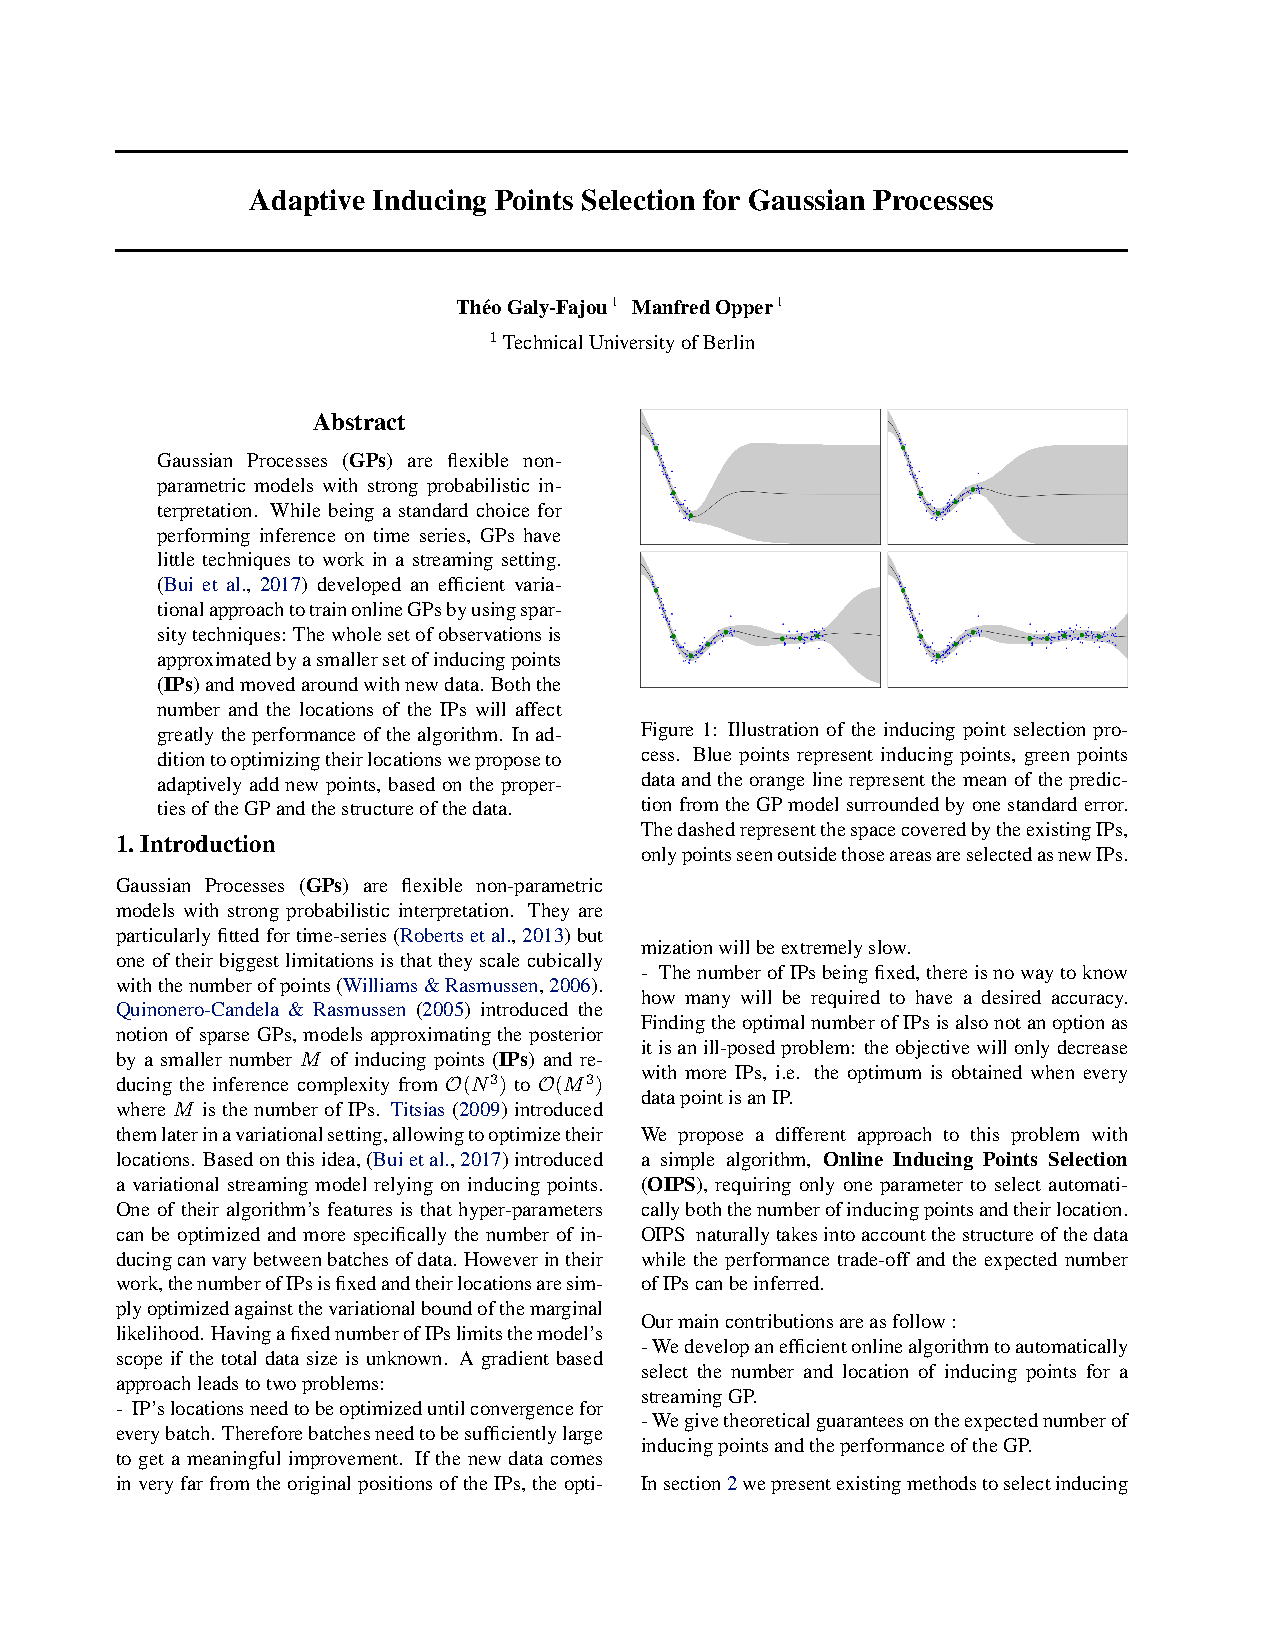
\includepdf[pages=-,pagecommand={},scale=0.95]{./papers/28_CameraReadySubmission_cl_workshop_onlinegp.pdf}

% \section{Evidence Estimation by Kullback-Leibler Integration for Flow-Based Methods}

% \textbf{\underline{Authors:}}\\
% Nikolai Zaki$^1$, Th\'eo Galy-Fajou$^1$, Manfred Opper$^1$\\
% \small{$^1$TU Berlin}

% \textbf{\underline{Details:}}\\
% Type: Workshop article
% Submitted: October 2020\\
% Accepted: December 2020\\
% URL : \url{https://openreview.net/forum?id=LclKtSfmf9I}\\
% Conference: 3rd Symposium on Advances in Approximate Bayesian Inference, 2020\\


% 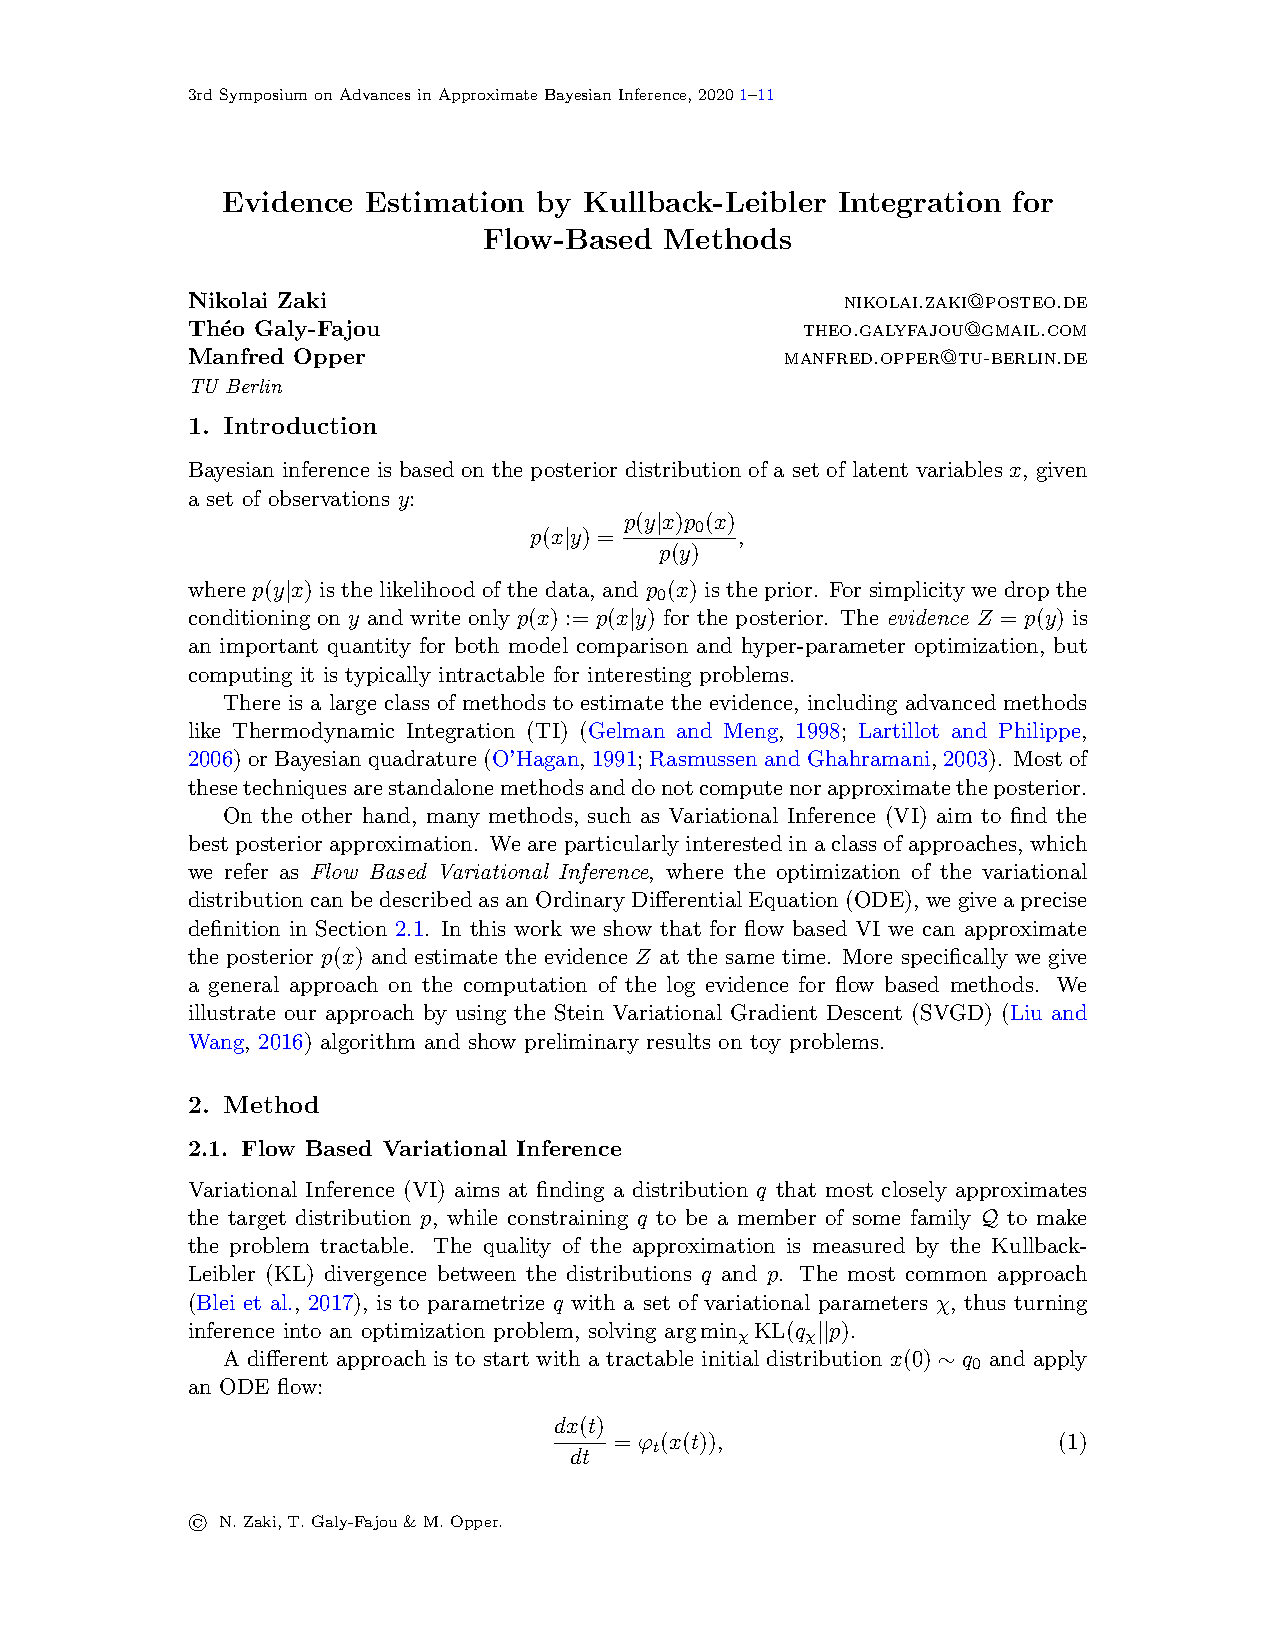
\includepdf[pages=-,pagecommand={},scale=0.95]{./papers/evidence_estimation_by_kullbac.pdf}
\end{appendices}

\end{document}
